% Self-contained source. Compile twice with pdflatex; no external figures or .bib needed.
\documentclass[10pt,a4paper]{article}
\usepackage[T1]{fontenc}
\usepackage[utf8]{inputenc}
\usepackage{lmodern}
\usepackage[margin=22mm,headheight=14pt]{geometry}
\usepackage{microtype,amsmath,amssymb,booktabs,array,tabularx,enumitem}
\usepackage{xcolor,tikz,fancyhdr}
\usetikzlibrary{arrows.meta,positioning}
\usepackage[colorlinks=true,linkcolor=teal!60!black,citecolor=teal!60!black,urlcolor=teal!60!black]{hyperref}
\hypersetup{pdftitle={When Should Cameras Ask Each Other? Selective Evidence Exchange for Dual-Camera Edge VLM Hazard Detection},pdfauthor={},pdfsubject={Research proposal with methodology, evaluation protocol, and submission risks}}
\definecolor{ink}{HTML}{183B4E}
\definecolor{pale}{HTML}{EEF4F6}
\pagestyle{fancy}
\fancyhf{}
\fancyhead[L]{\small\textcolor{ink}{Selective Evidence Exchange for Edge VLMs}}
\fancyhead[R]{\small Research proposal}
\fancyfoot[C]{\thepage}
\renewcommand{\headrulewidth}{0.3pt}
\setlength{\parindent}{0pt}
\setlength{\parskip}{5pt}
\setlength{\emergencystretch}{2em}
\setlist{nosep,leftmargin=1.5em}
\newcolumntype{Y}{>{\raggedright\arraybackslash}X}
\newcommand{\E}{\mathcal{E}}
\newcommand{\ind}{\mathbf{1}}
\newcommand{\note}[1]{\par\smallskip\noindent\colorbox{pale}{\parbox{\dimexpr\linewidth-2\fboxsep\relax}{#1}}\par\smallskip}

\begin{document}
\thispagestyle{empty}
{\Large\bfseries\color{ink} When Should Cameras Ask Each Other?\par}
\vspace{4pt}
{\large Selective Evidence Exchange for Dual-Camera\newline Edge VLM Hazard Detection\par}
\vspace{7pt}
{\small Research proposal and submission-risk assessment\hfill September 24, 2026\par}
\vspace{5pt}
\note{\small\textbf{Status.} This document proposes a research method and evaluation protocol. No implementation, dataset collection, or experimental results are claimed. Expected benefits are hypotheses to be tested.}

\begin{abstract}
Two cameras observing the same scene can expose complementary evidence of a hazardous event, yet continuous transmission of both video streams may be costly on edge devices. Independent alarms exploit view redundancy but do not necessarily combine evidence that is insufficient in either view alone. We propose to investigate selective, auditable evidence exchange between two locally deployed vision-language models (VLMs). Each device maintains a video buffer and structured observations, requests peer evidence when visibility or event evidence is inadequate, and verifies the event using time-aligned visual observations. The proposed policy explicitly considers confident false negatives, communication budgets, and response deadlines. Evaluation separates single-view-sufficient events from events judged to require both views, and compares against alarm-only fusion, budget-matched periodic exchange, local re-inference, and a centralized dual-view VLM. The main hypothesis is that evidence-aware requests improve deadline-constrained event recall at a fixed false-alarm allowance and communication budget. The proposal also identifies conditions under which this hypothesis would fail and the evidence required for a defensible paper submission.
\end{abstract}

\section{Introduction}
Fixed cameras in a retail-like environment often observe the same activity from different angles. One view may show a rapid change in body posture while shelving hides the subsequent body position; another may show a person on the floor but miss the preceding motion. These observations can support different explanations, including a fall, deliberate kneeling, or normal handling of objects. The research problem is to determine when exchanging additional evidence changes an event decision, and whether that change justifies its communication and latency cost.

Multi-camera VLM understanding already has clear precedents. CrossView studies reasoning over simultaneous camera streams, while SSMNBench distinguishes single-view sufficiency from multi-view necessity~\cite{crossview,ssmn}. Multi-camera anomaly detection also predates VLM-based systems~\cite{mcmil}. Consequently, combining two cameras with a VLM is not, by itself, a defensible novelty claim. Our narrower focus is online evidence acquisition between two edge-resident VLMs under explicit resource constraints.

A central distinction is between \emph{view redundancy} and \emph{evidence complementarity}. If camera B can independently detect an event missed by A, an alarm from B may already solve the system-level detection problem. A stronger collaboration claim concerns events whose decisive evidence is distributed across the two views, or cases where peer evidence rejects a false alarm without suppressing true events. We therefore evaluate the proposed policy against simple alarm fusion rather than only against individual cameras.

The intended contributions are: (1) an operational protocol separating independent detectability from cross-view evidence requirements; (2) a visibility- and evidence-aware request policy with bounded payloads and deadlines; and (3) an evaluation of recall, false alarms, delay, and actual network bytes under matched budgets. These are proposed contributions, not established findings. Neither a new metric nor a restatement of baseline errors will be presented as a theoretical result.

\newpage
\section{Related Work}
\subsection{Multi-camera and multi-view VLM understanding}
CrossView introduces multi-camera video question answering across four domains, including surveillance, with 6,000 questions and two to eight simultaneous streams~\cite{crossview}. It motivates cross-view integration, viewpoint selection, and temporal reasoning. Its benchmark focus does not establish a solution to distributed, deadline-constrained hazard detection. SSMNBench separates single-view-sufficient and multi-view-necessary questions and reports failures both from redundant views and from fragmented cross-view evidence~\cite{ssmn}. This distinction motivates our data stratification, although its image-based QA labels cannot directly substitute for online event annotations.

All-Angles Bench examines multi-view correspondence and camera-pose understanding~\cite{angles}. These difficulties caution against assuming that feeding additional images into a VLM automatically improves detection. They also motivate restricting the first study to fixed, calibrated scene zones instead of claiming general cross-camera identity resolution.

\subsection{Multi-camera anomaly detection and VLM-based VAD}
MC-MIL combines multiple-instance learning with multiple camera views and evaluates anomaly detection on a relabeled PETS-2009 dataset~\cite{mcmil}. It establishes that complementary camera observations can benefit anomaly detection without language-model reasoning. Its task and fusion design are relevant baselines, but its crowd-behavior setting differs from the proposed retail-like hazard scenarios.

LAVAD uses visual descriptions and language-model reasoning for training-free video anomaly detection~\cite{lavad}. VERA learns verbal guidance for a frozen VLM, showing how anomaly assessment can be organized through focused questions~\cite{vera}. Cerberus combines lightweight filtering and detailed VLM reasoning to reduce inference costs~\cite{cerberus}. These works motivate local evidence extraction and selective computation; their published performance does not determine our edge hardware throughput. Any offline temporal refinement must be removed or made causal before it is used in an online comparison.

Cascading multi-agent anomaly detection coordinates event-response and monitoring functions through a cascade~\cite{cascade}. Multi-agent orchestration is relevant to deployment, but role-based orchestration is distinct from proving that two camera-local VLMs combine mutually necessary visual evidence. We do not attribute a cross-view reasoning evaluation to that work.

\subsection{Communication-efficient cooperation}
Where2comm uses spatial confidence to select information for collaborative perception~\cite{where}. V2V-LLM studies multimodal language-model cooperation in connected-vehicle perception and driving~\cite{v2v}. These are substantive precedents for selective communication and semantic fusion. Adapting them to hazard detection requires a concrete mechanism and controlled evidence, not merely a change of application.

LatentMAS explores latent collaboration among language-model agents~\cite{latent}. Its reported reductions in generated tokens motivate alternative representations but do not establish a reduction in transmitted bytes between camera devices. Latent and visual-token exchange are therefore outside the initial method. Text, crops, and features also provide no automatic privacy guarantee.

\subsection{Scope of the claimed gap}
The targeted combination is local VLM inference on two devices, evidence-aware cross-view requests, causal hazard detection, and measured network and alarm costs. The reviewed sources motivate this combination but do not prove the absence of other methods. A submission must refresh the literature review and compare the actual mechanism against the closest selective-communication approaches. We make no claim to be the first multi-view VLM system, the first multi-agent VAD system, or the first uncertainty-triggered communication policy.

\newpage
\section{Our Methodology}
\subsection{Setting, assumptions, and observable event definitions}
Two fixed cameras $c\in\{A,B\}$ observe partially overlapping scene regions. Each edge device runs a VLM with the same frozen weights, retains a rolling video buffer, and executes a causal local pipeline. At reference time $t$, the available observation is
\begin{equation}
 x_c(t)=\{I_c(u):t-W<u\leq t\},
\end{equation}
where $W$ is a fixed past-context duration. No future frames are accessible. Clip duration, sampling frequency, resolution, model precision, and output limits are selected on development data and held fixed during testing.

For the first study, scene zones are mapped into both cameras during setup, and each queried zone contains at most one relevant actor or interaction group. Requests identify a shared zone, not a bounding box copied from the other camera. Local tracking may support crop extraction, but general cross-camera re-identification is not claimed. A planar mapping is used only where its geometric assumptions hold; an ambiguous correspondence falls back to a wider zone view or an explicit unresolved response.

Hazards are defined through observable actions and outcomes, such as a fall or forceful physical contact, with confusable normal activities included. Visual evidence alone does not establish hidden intent or legal categories such as theft. Event $e$ has a reference start $t_e$, end, class, scene zone, and supporting evidence intervals. Annotation instructions specify onset and alarm-matching tolerances before evaluation.

\subsection{Evidence requirements versus model failures}
Annotators assess each event using view A alone, view B alone, and both views. They label whether the task definition is supportable from each input, which observations support it, and where visibility is inadequate. To reduce hindsight leakage, single-view judgments are collected before joint-view review, preferably from separate annotators. Ambiguous cases are retained as uncertain and analyzed separately.

\begin{center}
\small
\begin{tabularx}{\linewidth}[t]{@{}>{\raggedright\arraybackslash}p{28mm}YY@{}}
\toprule
Stratum & Evidence condition & What a gain would support \\
\midrule
Redundant & Either view is sufficient. & Robustness or efficiency; not necessary cross-view reasoning. \\
One-view sufficient & Exactly one view is sufficient. & View selection, alarm routing, or false-alarm rejection. \\
Joint-view necessary & Neither view is sufficient, but the pair is sufficient. & The strongest test of evidence integration. \\
Unresolved & Even the pair is insufficient or disputed. & Appropriate abstention and limits of observability. \\
\bottomrule
\end{tabularx}
\end{center}

These labels are task- and annotation-protocol-dependent, not a proof of information-theoretic necessity. Separately, let $d_c(e;D)$ indicate whether the frozen single-camera baseline detects $e$ within deadline $D$. Cases with $d_A=0,d_B=1$ measure model-conditioned recoverability, but alarm-only fusion may already detect them. The subset $d_A=d_B=0$ is also model-dependent and may include fully observable events. It must not be equated with the independently annotated joint-view-necessary stratum.

\subsection{Constrained objective}
Let $T_e^\pi$ be the earliest valid system alarm for event $e$ under policy $\pi$, and let $T_e^\pi=\infty$ for a miss. The primary metric is
\begin{equation}
 R_D(\pi)=\frac{1}{|\E|}\sum_{e\in\E}\ind[T_e^\pi\leq t_e+D].
\end{equation}
We compare policies maximizing $R_D$ subject to false alarms per normal hour $F(\pi)\leq\alpha$ and transmitted bytes per hour $C(\pi)\leq B$. Thresholds are calibrated on held-out development data; test-set constraints are measured, not presumed satisfied. Results are reported across several $D$, $B$, and $\alpha$ settings rather than collapsed into an arbitrary weighted score.

\newpage
\subsection{Local observations and the request policy}
For each zone and clip, the local pipeline emits an event score, observed actions, a visibility state, evidence references, and a list of missing event predicates. Visibility takes explicit values such as visible, occluded, outside the field of view, or unresolved. A language-generated confidence score is not assumed calibrated. Its relationship to errors must be checked on development data, and it is only one input to the request policy.

The initial implementation uses an interpretable gate rather than an unspecified learned agent. For camera $c$, define normalized features $v_c$ for poor visibility, $m_c$ for missing event evidence, $u_c$ for score ambiguity, and $q_c$ for a lightweight activity candidate. Visibility and activity can use inexpensive detection, motion, or pose signals in addition to the VLM. The gate is
\begin{equation}
 g_c(t)=w_vv_c(t)+w_mm_c(t)+w_uu_c(t)+w_qq_c(t),\qquad w_j\geq0.
\end{equation}
The weights and threshold are selected from a predeclared small search space on development data under the communication constraint. They are not adjusted after observing test events. Crucially, visibility and missing-evidence terms can trigger a query even when the local hazard score is low. This makes confident false negatives an explicit test case rather than assuming all errors are uncertain.

Each device queries at most once per zone and decision window when $g_c(t)$ exceeds its threshold, the peer has a mapped view of the zone, a conservative reply-time estimate fits the configured request timeout, and sufficient byte credits remain. A token bucket limits transmission with a declared refill rate and burst allowance; the two devices receive fixed shares of the pair's budget. A request reserves a worst-case reply size as well as control-message overhead. Actual wire bytes determine compliance, and all budget overruns are reported.

Always-occluded regions could otherwise consume the budget continuously. A zone cooldown and bounded request frequency prevent repeated identical requests. These controls can themselves cause misses and are included in the ablation and failure analysis. If both local pipelines miss all useful cues, selective requests may never start. A low-rate probing variant is evaluated separately, with probes charged to the same budget.

\subsection{Request and reply contents}
A request contains a unique identifier, source camera, common scene-zone identifier, desired capture-time interval, clock-uncertainty bound, a short question about missing evidence, reply deadline, and payload cap. For example: ``During this interval, is the person's torso on the floor, and does the person return to standing?'' The question should solicit observations rather than ask the peer to endorse ``a fall occurred.''

The peer returns a bounded set of timestamped crops or wider zone images, brief factual observations, visibility states, and evidence identifiers. Sampling is deterministic in the initial method: fixed endpoint/intermediate samples from the requested interval, with a fixed crop-size and frame-count limit. More elaborate frame selection would introduce a second method and is deferred. A short sequence is retained for motion-dependent claims; a single static crop cannot establish an action trajectory.

Replies distinguish missing footage, insufficient visibility, ambiguous correspondence, and a negative observation made under adequate visibility. Reply generation cannot consult event labels or future frames. When the requested frames have expired from the buffer, the peer returns an explicit unavailable response. The requester never treats an unavailable reply as evidence that the scene is safe.

\note{\small\textbf{Method status.} The linear gate is a concrete starting design. Its novelty and effectiveness remain open. The essential ablation is whether visibility and evidence-deficit signals outperform a score-only gate under equal communication and compute budgets.}

\newpage
\subsection{Asynchronous alignment and evidence verification}
\begin{figure}[h]
\centering
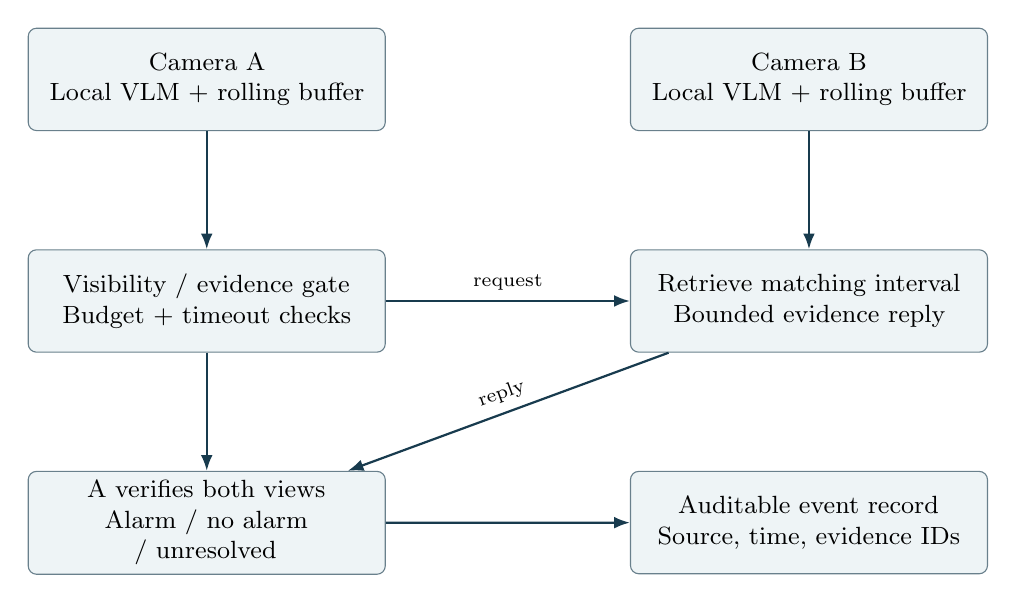
\begin{tikzpicture}[font=\small,box/.style={draw=ink!65,rounded corners=3pt,fill=pale,align=center,text width=43mm,minimum height=13mm},arr/.style={-{Latex[length=2mm]},thick,draw=ink}]
\node[box] (a) {Camera A\\Local VLM + rolling buffer};
\node[box,right=31mm of a] (b) {Camera B\\Local VLM + rolling buffer};
\node[box,below=15mm of a] (g) {Visibility / evidence gate\\Budget + timeout checks};
\node[box,below=15mm of b] (r) {Retrieve matching interval\\Bounded evidence reply};
\node[box,below=15mm of g] (v) {A verifies both views\\Alarm / no alarm / unresolved};
\node[box,below=15mm of r] (l) {Auditable event record\\Source, time, evidence IDs};
\draw[arr] (a)--(g);
\draw[arr] (b)--(r);
\draw[arr] (g)--node[above,font=\scriptsize]{request}(r);
\draw[arr] (r)--node[above,sloped,font=\scriptsize]{reply}(v);
\draw[arr] (g)--(v);
\draw[arr] (v)--(l);
\end{tikzpicture}
\caption{One request cycle. B can initiate the same process. Independent local alarms remain enabled and are evaluated as a separate baseline.}
\end{figure}

Capture time and completion time are logged separately. Camera timestamps are mapped to a shared reference clock using estimated offsets. If the residual offset uncertainty is bounded by $\epsilon$, the peer retrieves the requested interval expanded by $\epsilon$ on both ends and includes original timestamps. The buffer must cover past context plus the expected request age and clock margin. Tests vary capture-clock offsets separately from network and inference delays, because these produce different failures.

The requester processes a reply only after it actually arrives. It cannot backdate an alarm to the requested clip's capture time. If no valid reply arrives before the local timeout, it preserves its local decision or marks the event unresolved. Late replies may create a later, separately timestamped update, but cannot receive credit for meeting an earlier detection deadline. The request timeout uses known operational settings, not the unknown ground-truth event onset.

The requesting device performs one bounded verification pass using its own past clip and the returned visual evidence. Camera IDs and timestamps remain attached to every image. The verifier emits a hazard label, supporting evidence IDs, contradictory observations, and an unresolved flag. Observations from an occluded view do not veto positive evidence from a visible view merely because they report ``not seen.'' Descriptions are treated as fallible observations; visual support is required for decisive claims.

Both devices retain independent alarm capability. A verified local alarm is not withheld while waiting for a peer. Collaboration may add a new alarm or revise an unresolved assessment. Subsequent corrections are logged without erasing an already emitted false alarm from evaluation. A lightweight event collector deduplicates alarms by zone, class, and a preregistered time rule; it does not run an additional VLM. Its traffic is charged to every relevant system.

\subsection{Auditability and falsifiable hypotheses}
Each decision records model and prompt versions, request and reply IDs, source frames, capture and arrival times, missing predicates, payload bytes, and timeout status. This supports error attribution but does not guarantee that a generated explanation is faithful. Evidence support is independently checked on a labeled audit subset.

The main hypothesis is higher $R_D$ than alarm-only and budget-matched exchange baselines, especially on the joint-view-necessary stratum. Secondary hypotheses are improved false-alarm rejection and robustness to modest timing errors. Gains restricted to one-view-sufficient events support a narrower routing claim. Failure to outperform score-only triggering would weaken the case for the evidence-aware mechanism.

\newpage
\section{Planned Experimental Evaluation}
\subsection{Data, splits, and causal replay}
Record synchronized paired videos in controlled retail-like scenes, including staged falls and forceful interactions, matched normal actions, varied occlusions, and substantial normal operation. Annotate event intervals, scene zones, visibility, supporting evidence, and the evidence strata defined above. Staged incidents must be reported as staged. Broader deployment claims require additional environments or external validation. PETS-2009 can supplement the study with a distinct multi-camera activity setting; CrossView is only a capability diagnostic, not a substitute hazard-detection benchmark.

Split by recording session and, where feasible, actor and environment. Both views and all crops of one incident remain in the same split. Gate selection and score calibration use development data only. Online replay exposes frames according to capture and arrival times and includes measured inference queuing; processing a complete clip offline is not sufficient to establish real-time performance. Report inter-annotator agreement and retain uncertain evidence-sufficiency cases separately.

\subsection{Baselines and ablations}
\begin{center}
\small
\begin{tabularx}{\linewidth}[t]{@{}>{\raggedright\arraybackslash}p{36mm}Y@{}}
\toprule
System & Purpose and comparison condition \\
\midrule
Individual A and B & Report both. Select any preferred fixed camera on validation data, not per test event. Neither is a mathematical lower bound. \\
Alarm-only fusion & Each device sends compact positive alarms; system OR tests whether the peer could simply alert independently. \\
Continuous score fusion & Calibrated OR/max or mean scoring tests cheap decision fusion; system-level false alarms are calibrated jointly. \\
Periodic / random exchange & Same evidence format and verifier, with matched byte and additional-inference budgets. Isolates request selection. \\
Score-only request gate & Same protocol, using only score ambiguity. Isolates visibility and missing-evidence features. \\
Local extra inference & Re-analyze the same local evidence under matched additional compute. Tests whether gains require the other view. \\
Centralized dual-view VLM & Jointly processes timestamped views. Report unconstrained and bandwidth-matched variants; a strong comparator, not an upper bound. \\
Proposed exchange & Full gate, bounded replies, and evidence verification on a camera device. \\
Hindsight request reference & Uses event annotations to identify useful request opportunities. Diagnostic only, non-deployable, and not a proved upper bound. \\
\bottomrule
\end{tabularx}
\end{center}

Ablate visibility and missing-evidence terms, descriptions versus crops versus both, alignment handling, and bounded periodic probes. Keep the model, local sampling, event definitions, and extra-inference allowance fixed wherever applicable. A centralized system with different hardware is reported as a separate deployment configuration, not an equal-compute comparison. An additional model family is desirable before making model-agnostic claims.

\subsection{Metrics and stress tests}
Report deadline recall $R_D$ overall and by evidence stratum at validation-calibrated false-alarm targets, together with actual test false alarms per normal hour. Use a fixed event-matching and deduplication rule. Include confusable normal actions in calibration and testing. Conditional delay median and P95 are secondary: report the detection denominator so that misses cannot make a system appear faster.

Measure transmitted bytes once at the sender across both devices and the collector, including protocol overhead, control traffic, replies, and retries. Report bytes per hour, burst rates, per-event costs, and budget violations. Measure end-to-end wall-clock delay, queue length, memory, utilization, and sustained processing rate on the actual edge devices. Stress clock error, network delay, packet loss, inference variability, and request contention. Use session-clustered paired confidence intervals; repeated runs of the same few incidents do not create independent event samples.

\newpage
\section{Paper Submission Risks}
\subsection{Method novelty and the integration-only objection}
\textbf{Risk: high.} Confidence-based requests and selective communication have strong precedents. A linear gate, prompts, and a message queue may be judged an engineering combination; a recovery metric does not resolve this concern. A method claim requires demonstrated gains from visibility and missing-evidence signals over uncertainty-only and budget-matched policies. If absent, frame the work as a systems study or diagnostic benchmark and narrow its claims.

\subsection{Trivial recovery and failure to establish complementarity}
\textbf{Risk: high.} A peer that already detects the event can send an inexpensive alarm. Improvements over one camera alone would therefore be weak evidence of collaborative reasoning. The paper needs alarm-only fusion and independently annotated joint-view-necessary events. Show concrete cases where neither independent decision succeeds but correctly aligned peer evidence changes the result. Also report harmful exchanges, such as peer hallucinations that turn a correct local judgment into a false alarm. If all gains are routing gains, name that contribution explicitly.

\subsection{Small staged data and annotation leakage}
\textbf{Risk: high.} A small set of actors, camera positions, or scripted hazards can make performance depend on scene shortcuts. Joint-view knowledge can also leak into single-view sufficiency labels. Use session-level splits, matched normal behaviors, separate single-view judgments, and held-out layouts where possible. Report uncertain labels, agreement, event counts, and normal-video hours. Four event classes alone do not establish adequate scale. Broad surveillance claims require stronger coverage than a controlled two-camera proof of concept.

\subsection{Online validity, budget fairness, and edge feasibility}
\textbf{Risk: high until measured.} Future-frame access, hidden preprocessing, uncounted message overhead, or unmatched verifier calls can produce misleading gains. Audit causal replay and count the complete processing path. Report misses alongside latency, and queue growth alongside throughput. An inference configuration that cannot keep up with incoming clips must declare its frame-dropping or scheduling policy. Server-GPU results from prior work do not establish feasibility on the chosen edge device. Packet-level bytes and measured end-to-end delay are required to support deployment claims.

\subsection{Correspondence, trigger coverage, and trust}
\textbf{Risk: moderate to high.} Calibrated zones and a single relevant target simplify correspondence substantially. This is an explicit scope restriction, not a solution to re-identification. Confidently wrong local models may never request help; periodic probes can reduce but cannot eliminate that limitation under a finite budget. Clock errors can associate unrelated actions. Evidence references improve traceability but do not guarantee causal explanations or factual outputs. Evaluate visibility mistakes, absent replies, wrong-time replies, ambiguous targets, and contamination by incorrect peer descriptions.

\subsection{Submission readiness and responsible scope}
A defensible submission needs a reproducible causal implementation, a refreshed comparison with prior methods, auditable paired data, and budget-controlled gains with uncertainty estimates across sessions. No universal F1 threshold guarantees acceptance. An algorithmic contribution needs more than a functional pipeline; a systems contribution must substantiate sustained deployment and resource tradeoffs.

Record staged data with consenting participants and avoid real hazardous acts. Document access control, retention, and releases because crops and descriptions may identify people. The system provides decision support, not evidence of criminal intent. Submission readiness depends on the experiments above and cannot yet be claimed.

\newpage
\begin{thebibliography}{11}
\setlength{\itemsep}{7pt}
\small
\bibitem{crossview} S. Shah et al. \emph{CrossView: Can Vision-Language Models Reason Across Cameras?} ECCV 2026, as listed on the authors' arXiv record. \href{https://arxiv.org/abs/2608.15539}{arXiv:2608.15539}.

\bibitem{ssmn} T. Guo, C. Liu, L. Chen, and X. Yu. \emph{SSMNBench: Diagnosing Image-based Cross-View Human-Object Understanding via Single-View Sufficiency and Multi-View Necessity.} 2026. \href{https://arxiv.org/abs/2606.25634}{arXiv:2606.25634}.

\bibitem{angles} C.-H. Yeh et al. \emph{Seeing from Another Perspective: Evaluating Multi-View Understanding in MLLMs.} 2025. All-Angles Bench. \href{https://arxiv.org/abs/2504.15280}{arXiv:2504.15280}.

\bibitem{mcmil} S. S. L. Pereira and J. E. B. Maia. \emph{A MIL Approach for Anomaly Detection in Surveillance Videos from Multiple Camera Views.} 2023 preprint. \href{https://arxiv.org/abs/2307.00562}{arXiv:2307.00562}. The manuscript cites this inspected version rather than unverified numerical results from a later publication.

\bibitem{lavad} L. Zanella, W. Menapace, M. Mancini, Y. Wang, and E. Ricci. \emph{Harnessing Large Language Models for Training-free Video Anomaly Detection.} CVPR, pp. 18527--18536, 2024. \href{https://openaccess.thecvf.com/content/CVPR2024/html/Zanella_Harnessing_Large_Language_Models_for_Training-free_Video_Anomaly_Detection_CVPR_2024_paper.html}{CVF Open Access}.

\bibitem{vera} M. Ye, W. Liu, and P. He. \emph{VERA: Explainable Video Anomaly Detection via Verbalized Learning of Vision-Language Models.} CVPR, 2025. \href{https://arxiv.org/abs/2412.01095}{arXiv:2412.01095}.

\bibitem{cerberus} Y. Zheng, X. Shi, J. Chen, and Y. Shu. \emph{Cerberus: Real-Time Video Anomaly Detection via Cascaded Vision-Language Models.} 2025. \href{https://arxiv.org/abs/2510.16290}{arXiv:2510.16290}.

\bibitem{cascade} T. Rehman, G. De Gasperis, and A. Shmahell. \emph{Cascading Multi-Agent Anomaly Detection in Surveillance Systems via Vision-Language Models and Embedding-Based Classification.} 2026. \href{https://arxiv.org/abs/2601.06204}{arXiv:2601.06204}.

\bibitem{where} Y. Hu, S. Fang, Z. Lei, Y. Zhong, and S. Chen. \emph{Where2comm: Communication-Efficient Collaborative Perception via Spatial Confidence Maps.} NeurIPS, 2022. \href{https://arxiv.org/abs/2209.12836}{arXiv:2209.12836}.

\bibitem{v2v} H.-K. Chiu et al. \emph{V2V-LLM: Vehicle-to-Vehicle Cooperative Autonomous Driving with Multimodal Large Language Models.} ICRA, 2026; first preprint 2025. \href{https://arxiv.org/abs/2502.09980}{arXiv:2502.09980}.

\bibitem{latent} J. Zou et al. \emph{Latent Collaboration in Multi-Agent Systems.} ICML 2026, as listed on the authors' arXiv record; first preprint 2025. \href{https://arxiv.org/abs/2511.20639}{arXiv:2511.20639}.
\end{thebibliography}

\vspace{8pt}
\note{\small\textbf{Source and claim boundary.} Bibliographic metadata and the cited methodological descriptions were checked against primary paper records and available paper text. This is a focused review, not a systematic or exhaustive search. No unverified performance numbers are used as evidence for the proposed method. Conference status is included only where supported by the inspected record.}
\end{document}
